\section{Izvedba aplikacije}

  \subsection{PHP konfiguracija}

    Ova PHP skripta se obavezno \textit{includea} na vrhu svake druge PHP
    skripte. Sadrži neke osnovne PHP postavke.

    \lstinputlisting[language=PHP, alsolanguage=HTML, caption={
      PHP -- osnovna konfiguracija}]{config.php}

  \subsection{Recikliranje koda}

    Jedan od temeljnih principa programiranja je izbjeći lošu redundanciju u
    kodu (engl. \textit{DRY - Don't Repeat Yourself.}). Iz tog razloga sam kod
    aplikacije pisao vrlo organizirano i modularno, te pokušavao definirati
    metode i funkcije za kod koji se ponavlja.

    Npr. postoje klase u projektu \textit{UserModel} i \textit{DocumentModel}.
    \textit{UserModel} sadrži sve metode i atribute koje opisuju korisnika.
    Slično vrijedi i za \textit{DocumentModel} klasu.

    \subsubsection{\textit{Util} klasa}

      \textit{Util} klasa (engl. \textit{Utility}) sadrži statičke metode koje
      se često koriste na raznim mjestima u projektu, ali ne mogu se
      kategorizirati u klasu za sebe.

      \lstinputlisting[language=PHP, alsolanguage=HTML, caption={
          PHP -- Util klasa}]{Util.php}

    \subsubsection{\textit{DB} klasa}

      \textit{DB} klasa (engl. \textit{DataBase}) sadrži često korištene metode
      i svojstva vezane za upravljanje bazom podataka, koje su smještene u tzv.
      \textit{singleton} klasu.

      \lstinputlisting[language=PHP, caption={
          PHP -- DB klasa}]{DB.php}

      \subsubsection{Jezik aplikacije}

        Višejezičnost aplikacije je postignuta tako da su svi znakovni nizovi
        korišteni u aplikaciji organizirani u dvije slične PHP datoteke -
        lang\_en.php i lang\_hr.php. Obje datoteke sadrže asocijativno polje
        \textit{LANG} -- ključevi su isti, a vrijednosti prevedene.

        \lstinputlisting[language=PHP, caption={
          PHP -- Engleski znakovni nizovi}]{lang_en.php}

        \lstinputlisting[language=PHP, caption={
          PHP -- Hrvatski znakovni nizovi}]{lang_hr.php}

    \subsubsection{Osnovna struktura stranice}

    \begin{figure}[h]
      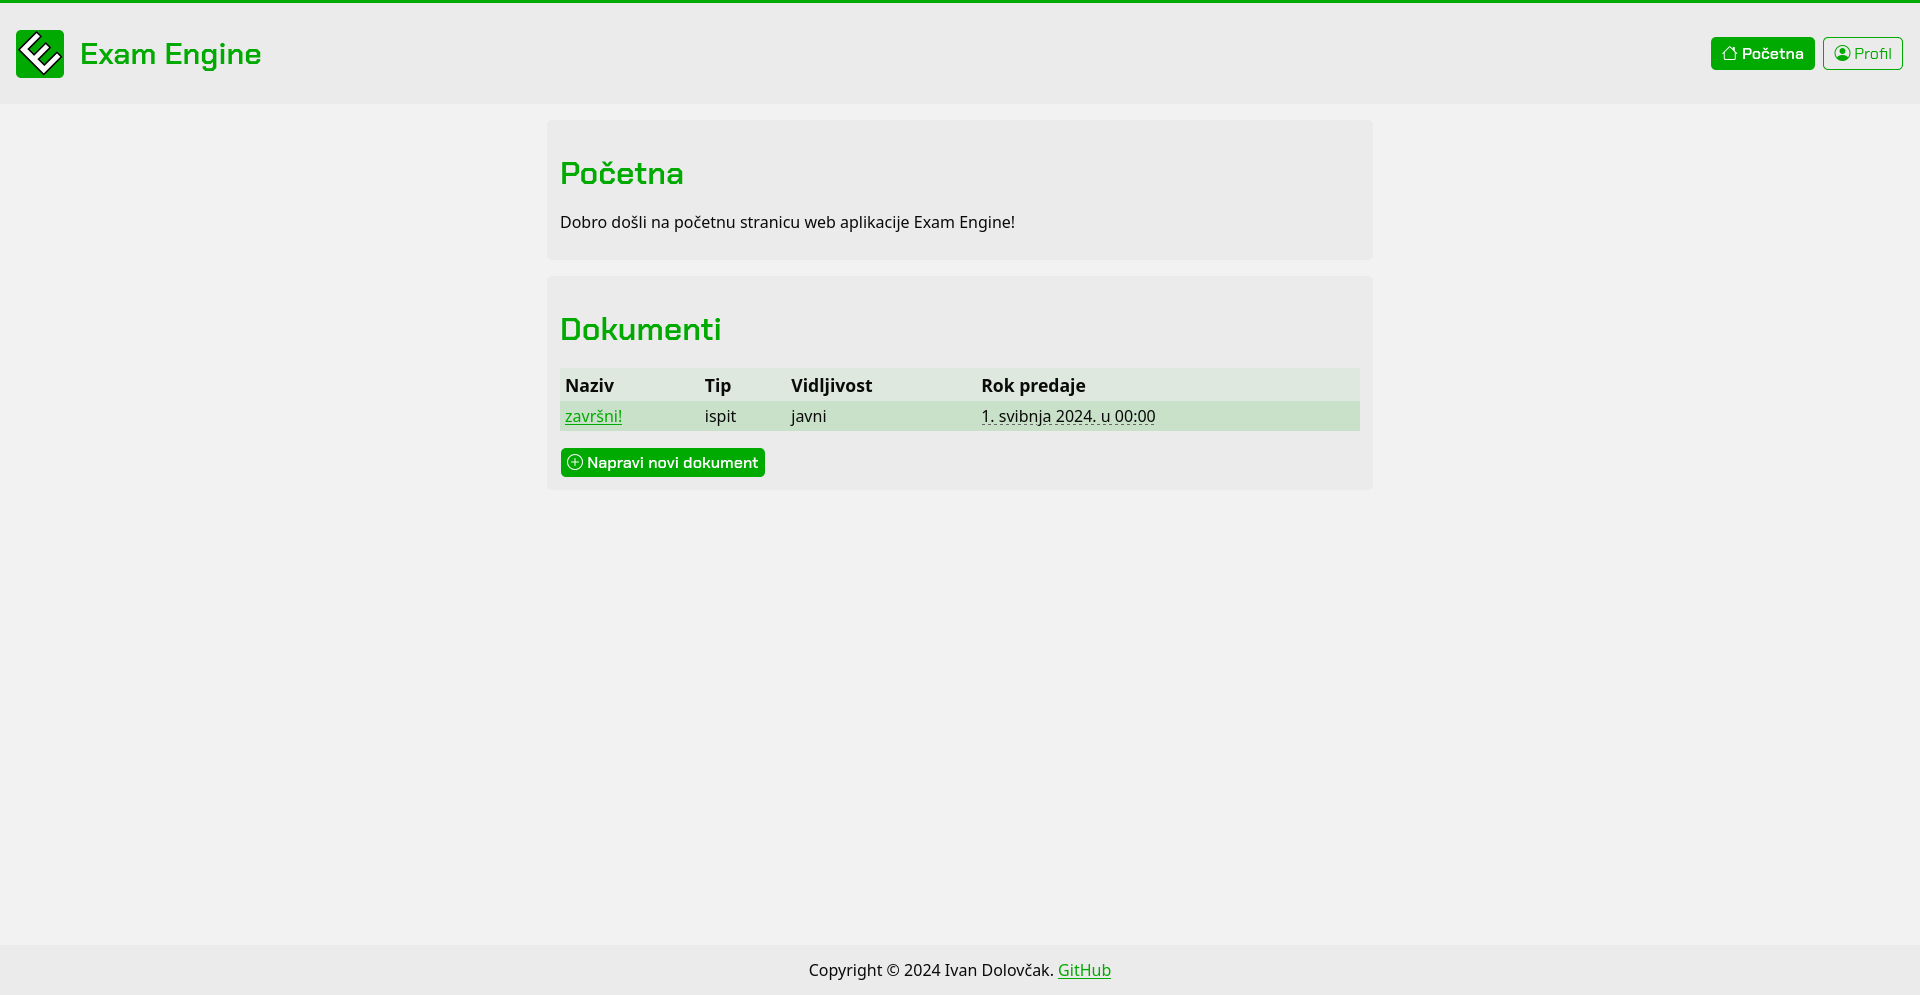
\includegraphics[width=\textwidth]{page_template}
      \caption{Početna stranica s popisom dokumenata.}
    \end{figure}

    Na svakoj stranici se ponavljaju zaglavlje i podnožje. Zaglavlje i podnožje
    stranice su stavljeni u zasebne datoteke (header.phtml i footer.phtml) te se
    na svakoj stranici \textit{includeaju}.

    Zaglavlje sadržava logotip aplikacije, naslov i navigator s poveznicama koje
    vode do glavnih stranica (engl. \textit{views}) aplikacije. Navigator
    mijenja svoj sadržaj ovisno o tome je li korisnik prijavljen. Ako nije,
    prikazuju se poveznice za registraciju i prijavu. Ako je, onda su te
    poveznice sakrivene.

    \subsection{Korisničke postavke (\textit{front-end})}

      \begin{figure}[h]
        \begin{center}
          \begin{subfigure}{0.65\textwidth}
            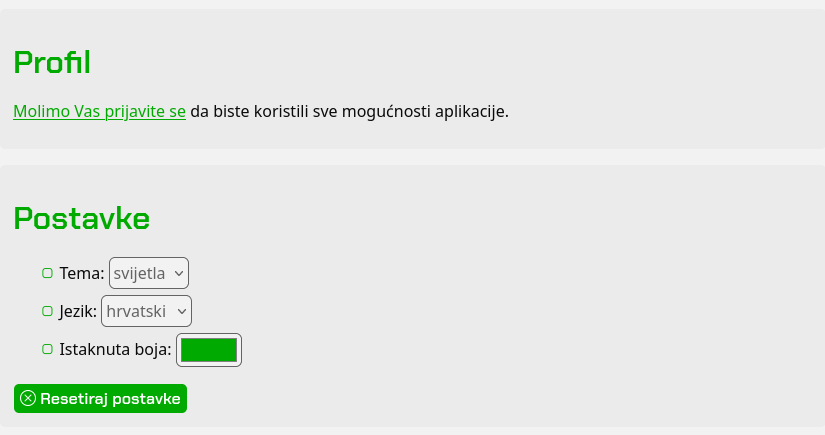
\includegraphics[width=\linewidth]{page_preferences_1}
          \end{subfigure}
          \\
          \begin{subfigure}{0.65\textwidth}
            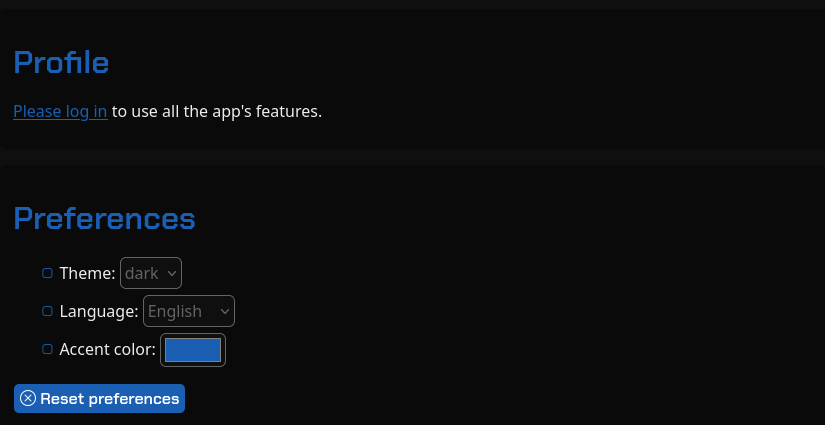
\includegraphics[width=\linewidth]{page_preferences_2}
          \end{subfigure}

          \caption{Prilagodljivost sučelja (profile.phtml)}
        \end{center}
      \end{figure}

      Izgled sučelja aplikacije je prilagodljiv korisniku.
      Korisničke postavke (engl. \textit{Preferences}) sastoje se od:

      \begin{itemize}
        \item teme (svijetla ili tamna),
        \item jezika (engleski ili hrvatsi)
        \item i boje isticanja (proizvoljna).
      \end{itemize}


    \subsection{Korisničke postavke (\textit{back-end})}

      Da bi mijenjao ove postavke prikaza, korisnik ne mora biti
      prijavljen u aplikaciju, jer se ove postavke spremaju u tzv. kolačić
      (engl. \textit{cookie}). Ako kolačić ne postoji (prva posjeta \textit{web}
      sjedištu), dodjeljuju se zadane (\textit{defaultne}) postavke (svijetla
      tema, zelena boja isticanja, engleski jezik).

      \subsubsection{\textit{Preferences} klasa}

        \lstinputlisting[language=PHP, caption={
          PHP -- Preferences klasa}]{Preferences.php}

  \subsection{Registracija korisnika (\textit{front-end})}

    \subsubsection{Prikaz obrasca za registraciju}

      \begin{figure}[h]
          \begin{subfigure}{0.5\textwidth}
            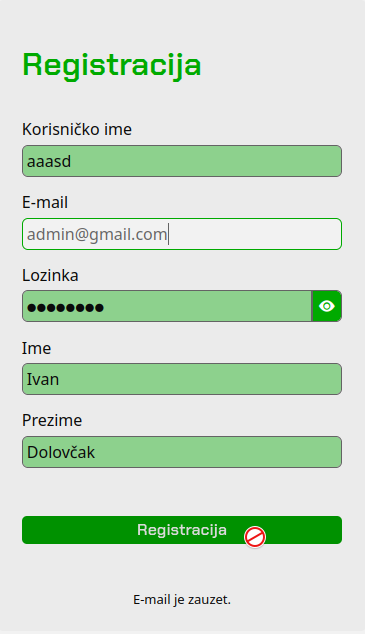
\includegraphics[width=0.9\linewidth]{form_register_1}
          \end{subfigure}
          \begin{subfigure}{0.5\textwidth}
            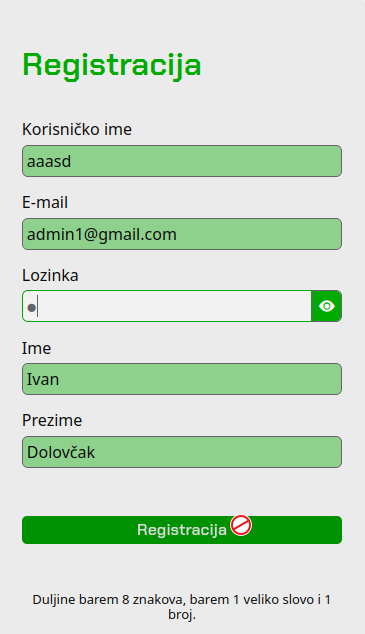
\includegraphics[width=0.9\linewidth]{form_register_2}
          \end{subfigure}

          \caption{Obrazac za registraciju -- validacija u realnom vremenu}
      \end{figure}

      Kako bi koristio sve mogućnosti aplikacije, korisnik mora biti
      registriran. To obavlja preko ovog obrasca, koji je intuitivan jer ima
      ugrađenu tzv. \textit{front-end} validaciju.

      Sva polja moraju biti popunjena i ispravna. Ukoliko neko polje nije ispravno,
      na dnu obrasca se u realnom vremenu (prije podnašanja obrasca) prikazuje
      povratna informacija korisniku te mu nije dozvoljeno podnašanje
      obrasca.

      Ukoliko je ispravno, polje se blago osjenča zelenom bojom. Ovo su uvjeti za
      ispravnost polja:

      \begin{itemize}
        \item Korisničko ime: Koristite velika i mala slova bez dijakritičkih
        znakova, brojeve i donje crte, duljine najmanje 4 znakova.
        \item Lozinka: Duljine barem 8 znakova, barem 1 veliko slovo i 1 broj.
        \item Ime i prezime: Duljine najmanje 3 znakova, bez brojeva.
        \item Korisničko ime i e-mail adresa ne smiju biti zauzeti
      \end{itemize}

      Valja napomenuti da su tijekom dizajniranja \textit{front-enda} uzete u
      obzir osnovne prakse pristupačnosti (engl. \textit{accessibility}):
      autofocus atributi, korištenje label elemenata koji su povezani sa svojim
      poljima za unos, te je za svako polje sačuvan tabindex atribut.

      \subsubsection{HTML/PHP struktura obrasca registracije}

        \lstinputlisting[language=PHP, alsolanguage=HTML, caption={
          HTML/PHP -- Obrazac za registraciju.}]{form_sign_up.phtml}

      \subsubsection{JS kod za validaciju}

        \lstinputlisting[language=JavaScript, caption={
          JS -- Live validacija forme.}]{form_validation.js}

  \subsection{Registracija korisnika (\textit{back-end})}

    \textit{Front-end} validaciju vrlo je lako zaobići, stoga je iz
    sigurnosnih razloga potrebno obaviti validaciju i u \textit{back-end}
    dijelu aplikacije.

    \subsubsection{Obrada obrasca za registraciju}

      \lstinputlisting[language=PHP, caption={
        PHP -- Obrada obrasca za registraciju.}]{sign_up.php}

    \subsubsection{Zapisivanje korisnika u bazu podataka}

      \lstinputlisting[language=PHP, alsolanguage=HTML, caption={
        PHP/SQL -- Zapisivanje korisnika u bazu podataka.}]{UserModelsignUp.php}
